\section{Whitney Music Box}
Aquesta fascinant aplicació està inspirada en les animacions de John Whitney (1917-1995), un cinematògraf que va explorar i va experimentar amb tècniques d'animació governades per normes mecàniques i matemàtiques, abans de l'era digital. Als anys cinquanta, Whitney va experimentar amb pèndols, engranatges, artefactes mecànics i primitius ordinadors analògics en combinació amb càmeres per produir pel·lícules curtes de línies i punts de llum, essent un pioner del vídeo com una forma plàstica de l'art abstracte. Als seixanta va adoptar els ordinadors digitals i va dedicar la seva carrera a l'art gràfic en ordinadors, amb curts i pel·lícules com Permutations (1968),   Arabesque (1976), o Moon Drum (1991).

L'any 1980, Whitney va publicar el llibre Digital Harmony, on descriu els seus experiments sobre la visualització de la música amb gràfics d'ordinador. Concretament, va explorar el que ell va anomenar ``moviment incremental'', una mena d'algorisme per decidir la posició de partícules, on cada partícula es ``mou'' des de l'anterior amb una norma molt simple. Una mena de norma de derivació que mitjançant la integració dóna l'increment a un comportament global que era originalment inesperat. Whitney donava al seu llibre un exemple de la seva espiral de moviment incremental. 

L'any 2006, el programador i animador a Disney Jim Bumgardner va agafar les idees de Whitney i va crear una aplicació interactiva amb l'addició de so a les espirals de Whitney. Bumgardner va crear el terme ``caixa de música de Whitney'' i l'aplicació ha sigut popular a internet des de llavors. 



\begin{figure}[h]
\centering
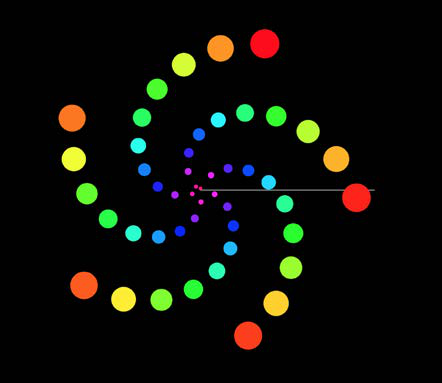
\includegraphics[width=0.5\textwidth]{Whitney_1}
\end{figure}

Matemàticament, l'aplicació es pot descriure força fàcilment. Cada punt es mou amb un centre concèntric i es mou a una velocitat angular proporcional al seu radi. Dit d'una altra manera: cada vegada que el punt situat a la zona més interna dóna una volta al voltant del cercle, el següent en dóna dues, el següent en dona tres, etc.

La referència general per la velocitat de rotació es pot controlar amb una rodeta de control. Cada punt reprodueix un to particular (assignat a l'escala cromàtica) quan el punt talla la línia horitzontal. Aquestes rotacions produeixen patrons canviants de l'espiral i acords quan diversos tons sonen alhora. La velocitat de rotació imposa una cadència rítmica de tons que reflecteixen la geometria del patró, evocant la consonància i dissonància de les notes de l'escala. 

Aquesta caixa de música permet visualitzar la ressonància harmònica i l'harmonia musical de forma molt agradable i aconsegueix que sigui un repte divertit però desafiant. Pot ser que trobis difícil de predir a què s'assemblaran els patrons musicals que en surtin cada vegada. Es tracta d'una eina que genera admiració i resulta fins i tot hipnòtica.


\begin{sectcredits}
\item[Autor del mòdul:] Eric Londaits (IMAGINARY). Inspirat en la implementació de Jürgen Richter-Gebert.

\item[Text:] Eric Londaits i Daniel Ramos (IMAGINARY).

\item[Referències:] \strut
\noindent \begin{itemize}[leftmargin=*]
\item \url{https://krazydad.com/blog/2006/04/23/visual-harmony}

\item \url{https://boingboing.net/2016/04/11/john-whitney-music-box-a-psyc.html}

\item \url{https://jbum.com/papers/whitney_paper.pdf}

\item John Whitney. \emph{Digital Harmony: On the Complementarity of Music and Visual Art}. Byte Books / McGraw-Hill (1980). \\
\url{https://archive.org/details/DigitalHarmony_201611}

\end{itemize}
\end{sectcredits}
